\section{Méthodes possibles pour la virtualisation légère}
\label{section:emulation}

Il existe actuellement deux méthodes permettant de faire de la virtualisation
légère. La première est une émulation par limitation ou dégradation également
appelée virtualisation standard et la seconde est une émulation par
interception.

\begin{figure}[H]
  \centering 
  \begin{subfigure}{0.3\textwidth}
    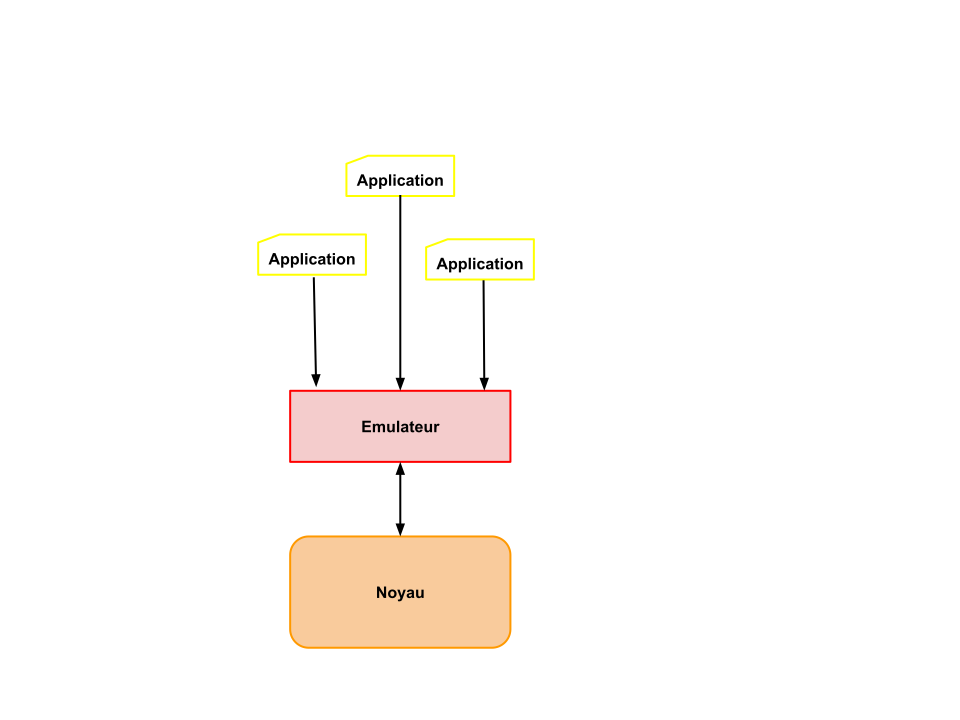
\includegraphics[scale=0.35]{Pictures/png/Virtualisation_limitation}
  \end{subfigure}
  \begin{subfigure}{0.3\textwidth}
    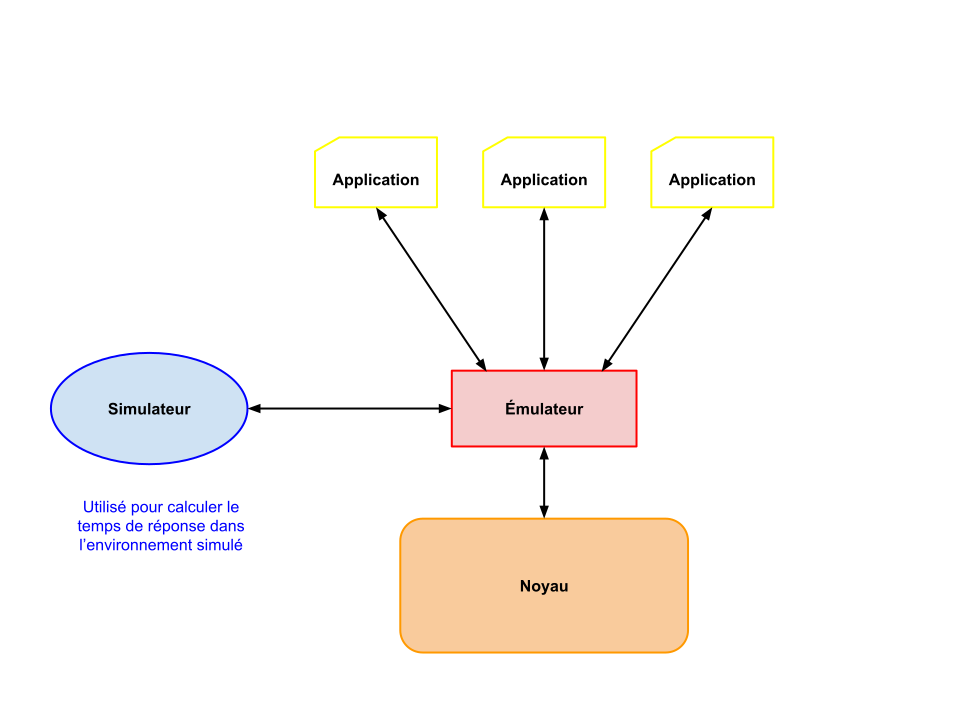
\includegraphics[scale=0.3]{Pictures/png/Virtualisation_interception}
  \end{subfigure}
  \caption{Virtualisation par limitation (à gauche) et par interception (à
    droite)}
  \label{TYPE_VIRTUALISATION}
\end{figure}









